\subsection{Lịch trình thực hiện và đường cơ sở chi phí (Cost Baseline)}
\label{sec:schedule-baseline}
Lịch trình chi tiết và Cost Baseline được xây dựng dựa trên 331,6 giờ công đã cân bằng tại Mục \ref{sec:resource-allocation}, bao gồm đầy đủ các tác vụ ứng phó rủi ro RA01--RA06. Dự án khởi động ngày 26/10/2026, bàn giao ngày 03/12/2026 và kết thúc ngày 06/12/2026.
\subsubsection{Quy ước lập lịch}
Lịch trình tuân thủ các quy tắc sau:
\begin{itemize}
    \item \textbf{Khung thời gian:} Tuần làm việc từ thứ Hai đến Chủ nhật, bao gồm 12 cửa sổ P1/P2 từ thứ Hai đến thứ Bảy.
    \item \textbf{Mối quan hệ tiền nhiệm:} Áp dụng dạng Finish-to-Start (FS) ở phiên tiếp theo.
    \item \textbf{Đồng bộ Milestone:} Milestone CP1 kiểm tra Increment 1 sau khi hoàn thành A06 và RA06.
\end{itemize}
\subsubsection{Lịch thực hiện hoạt động chi tiết}
\begingroup\small
\setlength{\tabcolsep}{4pt}\renewcommand{\arraystretch}{1.15}
\begin{longtable}{@{}p{.075\linewidth}p{.255\linewidth}p{.245\linewidth}>{\raggedleft\arraybackslash}p{.06\linewidth}p{.085\linewidth}p{.085\linewidth}@{}}
\caption{Lịch thực hiện chi tiết các hoạt động dự án}\label{tab:dates}\\
\toprule
\textbf{Mã} & \textbf{Hoạt động} & \textbf{Tiền nhiệm} & \textbf{Giờ} & \textbf{Bắt đầu} & \textbf{Kết thúc} \\
\midrule\endfirsthead
\toprule
\textbf{Mã} & \textbf{Hoạt động} & \textbf{Tiền nhiệm} & \textbf{Giờ} & \textbf{Bắt đầu} & \textbf{Kết thúc} \\
\midrule\endhead
\midrule\multicolumn{6}{r}{\textit{Còn tiếp}}\\\endfoot
\bottomrule\endlastfoot
A01 & Thiết kế CSDL, giao diện, API & --- & 16,0 & 26/10 & 28/10 \\
A02.1 & Test case Increment 1 & --- & 5,0 & 27/10 & 02/11 \\
A02.2 & Test case Increment 2 & A01 & 3,5 & 02/11 & 10/11 \\
A02.3 & Test case Increment 3 & A01 & 3,5 & 28/10 & 10/11 \\
A03 & Thiết lập môi trường triển khai & G04, A01 & 8,0 & 29/10 & 30/10 \\
A04.1 & Dữ liệu thử Increment 1 & A01, A02.1 & 3,5 & 03/11 & 03/11 \\
A05.1 & Lập trình Tài khoản, phân quyền & A03 & 18,0 & 02/11 & 04/11 \\
A05.2 & Lập trình Quản lý sự kiện & A03 & 18,0 & 30/10 & 03/11 \\
A06 & Kiểm thử, sửa lỗi Increment 1 & A05.1, A05.2, A04.1, A02.1 & 10,0 & 05/11 & 09/11 \\
A07.1 & Lập trình Đăng ký, hủy, sức chứa & A06, RA06 & 22,0 & 09/11 & 11/11 \\
A07.2 & Lập trình Danh sách chờ FIFO & A07.1, RA01 & 14,0 & 12/11 & 16/11 \\
A07.3 & Lập trình Email thông báo & A07.2, RA03 & 6,0 & 17/11 & 17/11 \\
A08 & Kiểm thử, sửa lỗi Increment 2 & A07.3, A02.2, BL1 & 13,0 & 18/11 & 19/11 \\
A09.1 & Lập trình Điểm danh QR & A08, RA04 & 12,0 & 21/11 & 24/11 \\
A09.2 & Lập trình Điểm danh thủ công & A08 & 10,0 & 20/11 & 23/11 \\
A10.1 & Lập trình Báo cáo cơ bản & A08 & 13,0 & 20/11 & 21/11 \\
A10.2 & Lập trình Xuất CSV/Excel & A10.1 & 5,0 & 23/11 & 23/11 \\
A11 & Tích hợp, triển khai nghiệm thu & A09.1, A09.2, A10.2, RA02 & 7,0 & 24/11 & 25/11 \\
A12.1 & Integration Test & A11, A02.3, BL1 & 14,0 & 26/11 & 27/11 \\
A12.2 & Đo chỉ tiêu, chốt Evidence & A12.1, RA05 & 8,0 & 27/11 & 30/11 \\
A14.1 & Soạn thảo User Guide & A11 & 3,0 & 25/11 & 30/11 \\
A15.1 & Tổng hợp số liệu đánh giá & A08 & 2,0 & 20/11 & 20/11 \\
A15.2 & Chốt đánh giá và bài học & A12.2, G07, A15.1 & 6,0 & 30/11 & 30/11 \\
A16 & Kế hoạch đóng và bàn giao & BL2, A15.2 & 5,0 & 01/12 & 01/12 \\
A17 & Demo và bàn giao sản phẩm & A18.2 & 5,0 & 03/12 & 03/12 \\
A18.1 & Tổng hợp bản thảo báo cáo & G07 & 2,5 & 10/11 & 10/11 \\
A18.2 & Chốt báo cáo quản lý dự án & A16, A19.2, A18.1 & 4,5 & 02/12 & 02/12 \\
A19.1 & Ghi nhận đóng góp, chuẩn bị demo & A06 & 2,5 & 17/11 & 21/11 \\
A19.2 & Hoàn thiện Reflection và diễn tập & A12.2, A19.1 & 2,5 & 01/12 & 01/12 \\
BL1 & Dữ liệu thử Increment 2, 3 & A01, A02.2, A02.3 & 3,5 & 11/11 & 11/11 \\
BL2 & Chốt phiên bản, xác minh User Guide & A12.2, A14.1 & 4,0 & 30/11 & 01/12 \\
G02 & Rà soát sản phẩm và phụ thuộc & --- & 10,0 & 26/10 & 26/10 \\
G03 & Ước lượng, lập kế hoạch lịch trình & G02 & 11,0 & 27/10 & 28/10 \\
G04 & Phê duyệt Project Baseline V1.0 & G03 & 4,0 & 29/10 & 29/10 \\
G05 & Theo dõi và kiểm soát tiến độ & Định kỳ sau G04 & 30,0 & 30/10 & 27/11 \\
G06 & Rà soát và kiểm soát rủi ro & Dữ liệu G05 & 7,5 & 31/10 & 28/11 \\
G07 & Phân tích và quản lý thay đổi & G04 & 8,0 & 04/11 & 09/11 \\
RA01 & Thử nghiệm tải đồng thời & A03 & 2,5 & 09/11 & 09/11 \\
RA02 & Thử nghiệm triển khai AWS Lightsail & A05.1 & 2,5 & 05/11 & 05/11 \\
RA03 & Thử nghiệm dịch vụ Email & A03 & 1,0 & 02/11 & 02/11 \\
RA04 & Thử nghiệm sinh, quét mã QR & A01 & 2,0 & 02/11 & 09/11 \\
RA05 & Thử nghiệm hiệu năng báo cáo & A10.1 & 1,9 & 23/11 & 23/11 \\
RA06 & Làm rõ yêu cầu kỹ thuật & A05.2 & 1,2 & 09/11 & 09/11 \\
\end{longtable}\endgroup
\subsubsection{Lịch phân bổ giờ công theo tuần (Effort Time-Phasing)}
Bảng \ref{tab:ledger} thể hiện lịch phân bổ giờ công của từng tác vụ qua 6 tuần. Dữ liệu này phục vụ theo dõi tiến độ và hạch toán chi phí nhân sự theo tuần.
\begin{table}[H]
\centering
\caption{Lịch phân bổ giờ công theo hoạt động và tuần (Đơn vị: Giờ công)}\label{tab:ledger}
\begingroup\footnotesize
\setlength{\tabcolsep}{2pt}\renewcommand{\arraystretch}{1.18}
\begin{minipage}[t]{.46\linewidth}
\vspace{0pt}\centering
\begin{tabular*}{\linewidth}{@{\extracolsep{\fill}}lrrrrrrr@{}}
\toprule
\textbf{Mã} & \textbf{T1} & \textbf{T2} & \textbf{T3} & \textbf{T4} & \textbf{T5} & \textbf{T6} & \textbf{Tổng} \\
\midrule
A01 & 16,0 & 0,0 & 0,0 & 0,0 & 0,0 & 0,0 & 16,0 \\
A02.1 & 2,0 & 3,0 & 0,0 & 0,0 & 0,0 & 0,0 & 5,0 \\
A02.2 & 0,0 & 2,0 & 1,5 & 0,0 & 0,0 & 0,0 & 3,5 \\
A02.3 & 1,5 & 0,0 & 2,0 & 0,0 & 0,0 & 0,0 & 3,5 \\
A03 & 8,0 & 0,0 & 0,0 & 0,0 & 0,0 & 0,0 & 8,0 \\
A04.1 & 0,0 & 3,5 & 0,0 & 0,0 & 0,0 & 0,0 & 3,5 \\
A05.1 & 0,0 & 18,0 & 0,0 & 0,0 & 0,0 & 0,0 & 18,0 \\
A05.2 & 4,0 & 14,0 & 0,0 & 0,0 & 0,0 & 0,0 & 18,0 \\
A06 & 0,0 & 8,0 & 2,0 & 0,0 & 0,0 & 0,0 & 10,0 \\
A07.1 & 0,0 & 0,0 & 22,0 & 0,0 & 0,0 & 0,0 & 22,0 \\
A07.2 & 0,0 & 0,0 & 10,9 & 3,1 & 0,0 & 0,0 & 14,0 \\
A07.3 & 0,0 & 0,0 & 0,0 & 6,0 & 0,0 & 0,0 & 6,0 \\
A08 & 0,0 & 0,0 & 0,0 & 13,0 & 0,0 & 0,0 & 13,0 \\
A09.1 & 0,0 & 0,0 & 0,0 & 4,4 & 7,6 & 0,0 & 12,0 \\
A09.2 & 0,0 & 0,0 & 0,0 & 8,7 & 1,3 & 0,0 & 10,0 \\
A10.1 & 0,0 & 0,0 & 0,0 & 13,0 & 0,0 & 0,0 & 13,0 \\
A10.2 & 0,0 & 0,0 & 0,0 & 0,0 & 5,0 & 0,0 & 5,0 \\
A11 & 0,0 & 0,0 & 0,0 & 0,0 & 7,0 & 0,0 & 7,0 \\
A12.1 & 0,0 & 0,0 & 0,0 & 0,0 & 14,0 & 0,0 & 14,0 \\
A12.2 & 0,0 & 0,0 & 0,0 & 0,0 & 5,8 & 2,2 & 8,0 \\
A14.1 & 0,0 & 0,0 & 0,0 & 0,0 & 2,8 & 0,2 & 3,0 \\
A15.1 & 0,0 & 0,0 & 0,0 & 2,0 & 0,0 & 0,0 & 2,0 \\
\bottomrule
\end{tabular*}
\end{minipage}\hfill
\begin{minipage}[t]{.46\linewidth}
\vspace{0pt}\centering
\begin{tabular*}{\linewidth}{@{\extracolsep{\fill}}lrrrrrrr@{}}
\toprule
\textbf{Mã} & \textbf{T1} & \textbf{T2} & \textbf{T3} & \textbf{T4} & \textbf{T5} & \textbf{T6} & \textbf{Tổng} \\
\midrule
A15.2 & 0,0 & 0,0 & 0,0 & 0,0 & 0,0 & 6,0 & 6,0 \\
A16 & 0,0 & 0,0 & 0,0 & 0,0 & 0,0 & 5,0 & 5,0 \\
A17 & 0,0 & 0,0 & 0,0 & 0,0 & 0,0 & 5,0 & 5,0 \\
A18.1 & 0,0 & 0,0 & 2,5 & 0,0 & 0,0 & 0,0 & 2,5 \\
A18.2 & 0,0 & 0,0 & 0,0 & 0,0 & 0,0 & 4,5 & 4,5 \\
A19.1 & 0,0 & 0,0 & 0,0 & 2,5 & 0,0 & 0,0 & 2,5 \\
A19.2 & 0,0 & 0,0 & 0,0 & 0,0 & 0,0 & 2,5 & 2,5 \\
BL1 & 0,0 & 0,0 & 3,5 & 0,0 & 0,0 & 0,0 & 3,5 \\
BL2 & 0,0 & 0,0 & 0,0 & 0,0 & 0,0 & 4,0 & 4,0 \\
G02 & 10,0 & 0,0 & 0,0 & 0,0 & 0,0 & 0,0 & 10,0 \\
G03 & 11,0 & 0,0 & 0,0 & 0,0 & 0,0 & 0,0 & 11,0 \\
G04 & 4,0 & 0,0 & 0,0 & 0,0 & 0,0 & 0,0 & 4,0 \\
G05 & 6,0 & 6,0 & 6,0 & 6,0 & 6,0 & 0,0 & 30,0 \\
G06 & 1,0 & 1,5 & 1,5 & 1,5 & 2,0 & 0,0 & 7,5 \\
G07 & 0,0 & 3,0 & 5,0 & 0,0 & 0,0 & 0,0 & 8,0 \\
RA01 & 0,0 & 0,0 & 2,5 & 0,0 & 0,0 & 0,0 & 2,5 \\
RA02 & 0,0 & 2,5 & 0,0 & 0,0 & 0,0 & 0,0 & 2,5 \\
RA03 & 0,0 & 1,0 & 0,0 & 0,0 & 0,0 & 0,0 & 1,0 \\
RA04 & 0,0 & 1,5 & 0,5 & 0,0 & 0,0 & 0,0 & 2,0 \\
RA05 & 0,0 & 0,0 & 0,0 & 0,0 & 1,9 & 0,0 & 1,9 \\
RA06 & 0,0 & 0,0 & 1,2 & 0,0 & 0,0 & 0,0 & 1,2 \\
\bottomrule
\end{tabular*}
\end{minipage}
\endgroup
\end{table}

Tổng công sức phân bổ từ T1 đến T6 lần lượt là 63,5; 64,0; 61,1; 60,2; 53,4 và 29,4 giờ công, tương ứng tổng cộng 331,6 giờ công.

\subsubsection{Danh mục Milestones kế hoạch}
\begingroup\small
\setlength{\tabcolsep}{4pt}\renewcommand{\arraystretch}{1.15}
\begin{longtable}{@{}p{.13\linewidth}p{.13\linewidth}p{.10\linewidth}p{.505\linewidth}@{}}
\caption{Danh mục Milestones kế hoạch}\label{tab:milestones}\\
\toprule
\textbf{Milestone} & \textbf{Tác vụ trước} & \textbf{Ngày} & \textbf{Điều kiện nghiệm thu \& Tiêu chí} \\
\midrule\endfirsthead
\toprule
\textbf{Milestone} & \textbf{Tác vụ trước} & \textbf{Ngày} & \textbf{Điều kiện nghiệm thu \& Tiêu chí} \\
\midrule\endhead
\midrule\multicolumn{4}{r}{\textit{Còn tiếp}}\\\endfoot
\bottomrule\endlastfoot
CPD & A01 & 28/10 & Hoàn thành rà soát thiết kế CSDL, UI và API specification. \\
CP0 & G04 & 29/10 & Phê duyệt Project Baseline V1.0. \\
CP1 & A06 & 09/11 & Increment 1 đạt yêu cầu kiểm thử; hoàn thành tác vụ RA06. \\
CP2 & A08 & 19/11 & Increment 2 đạt yêu cầu kiểm thử chức năng và Regression Test. \\
CP3 & A11 & 25/11 & Build tích hợp hoàn tất trên môi trường AWS Lightsail. \\
CP4 & A12.2 & 30/11 & Hoàn thành kiểm thử nghiệm thu, đạt chỉ tiêu và Quality Evidence. \\
CP5 & A18.2 & 02/12 & Rà soát toàn bộ hồ sơ bàn giao và phiên bản phần mềm. \\
CP6 & A17 & 03/12 & Demo và bàn giao sản phẩm chính thức. \\
Hạn nộp & --- & 06/12 & Nộp đầy đủ bộ hồ sơ dự án theo quy định. \\
\end{longtable}\endgroup
\subsubsection{Biểu đồ Gantt}
Lịch trình dự án được trực quan hóa qua các biểu đồ Gantt (Hình \ref{fig:gantt1}, \ref{fig:gantt2} và \ref{fig:ganttra}). Các thanh biểu diễn thời gian thực hiện tác vụ; các tác vụ thuộc Critical Path được đánh dấu nổi bật để tập trung theo dõi.
\begin{figure}[H]
\centering
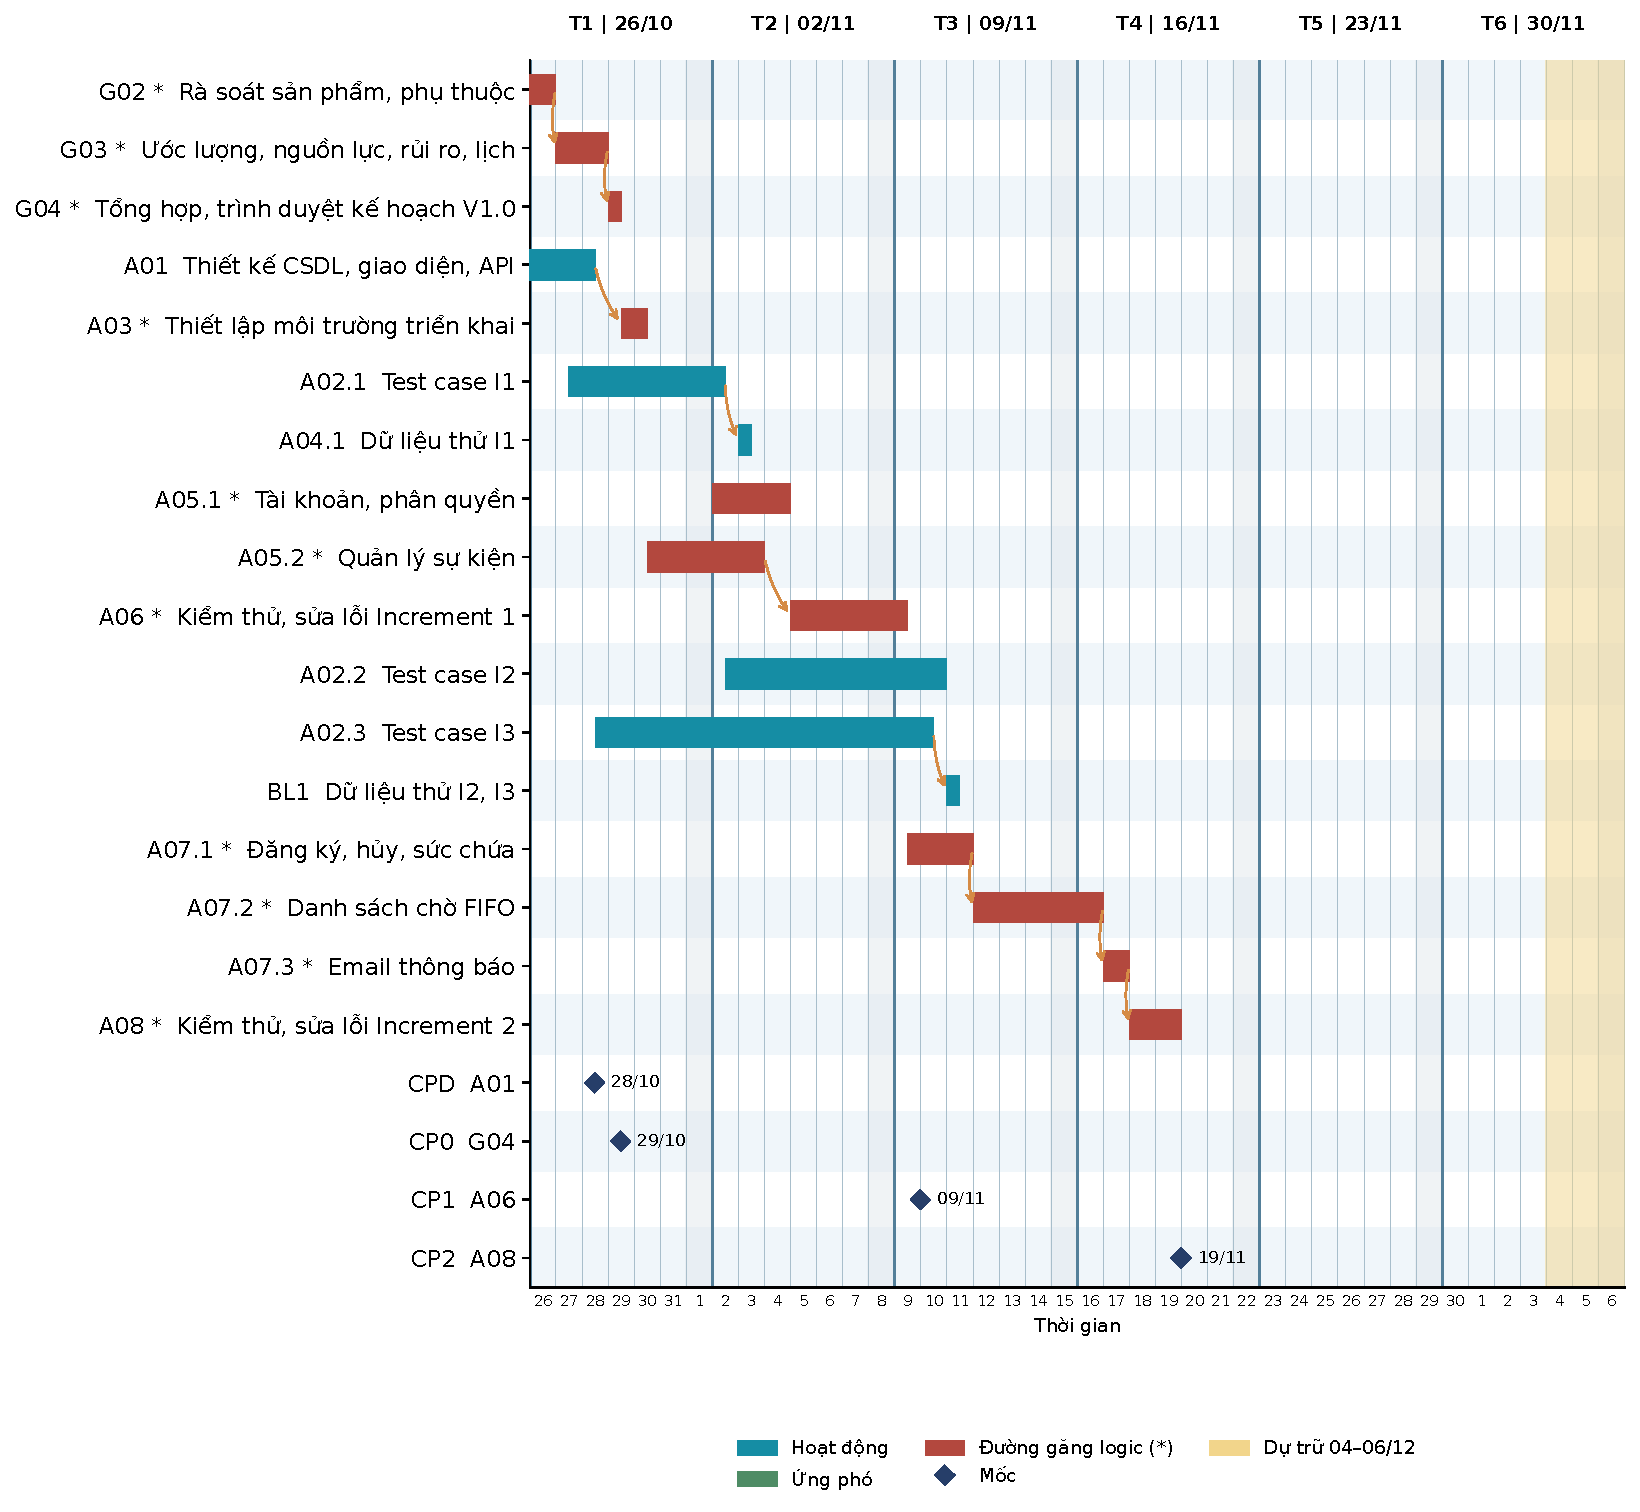
\includegraphics[width=\linewidth,height=.85\textheight,keepaspectratio]{Images/gantt_1.pdf}
\caption{Biểu đồ Gantt tiến độ Increment 1 và Increment 2}
\label{fig:gantt1}
\end{figure}
\begin{figure}[H]
\centering
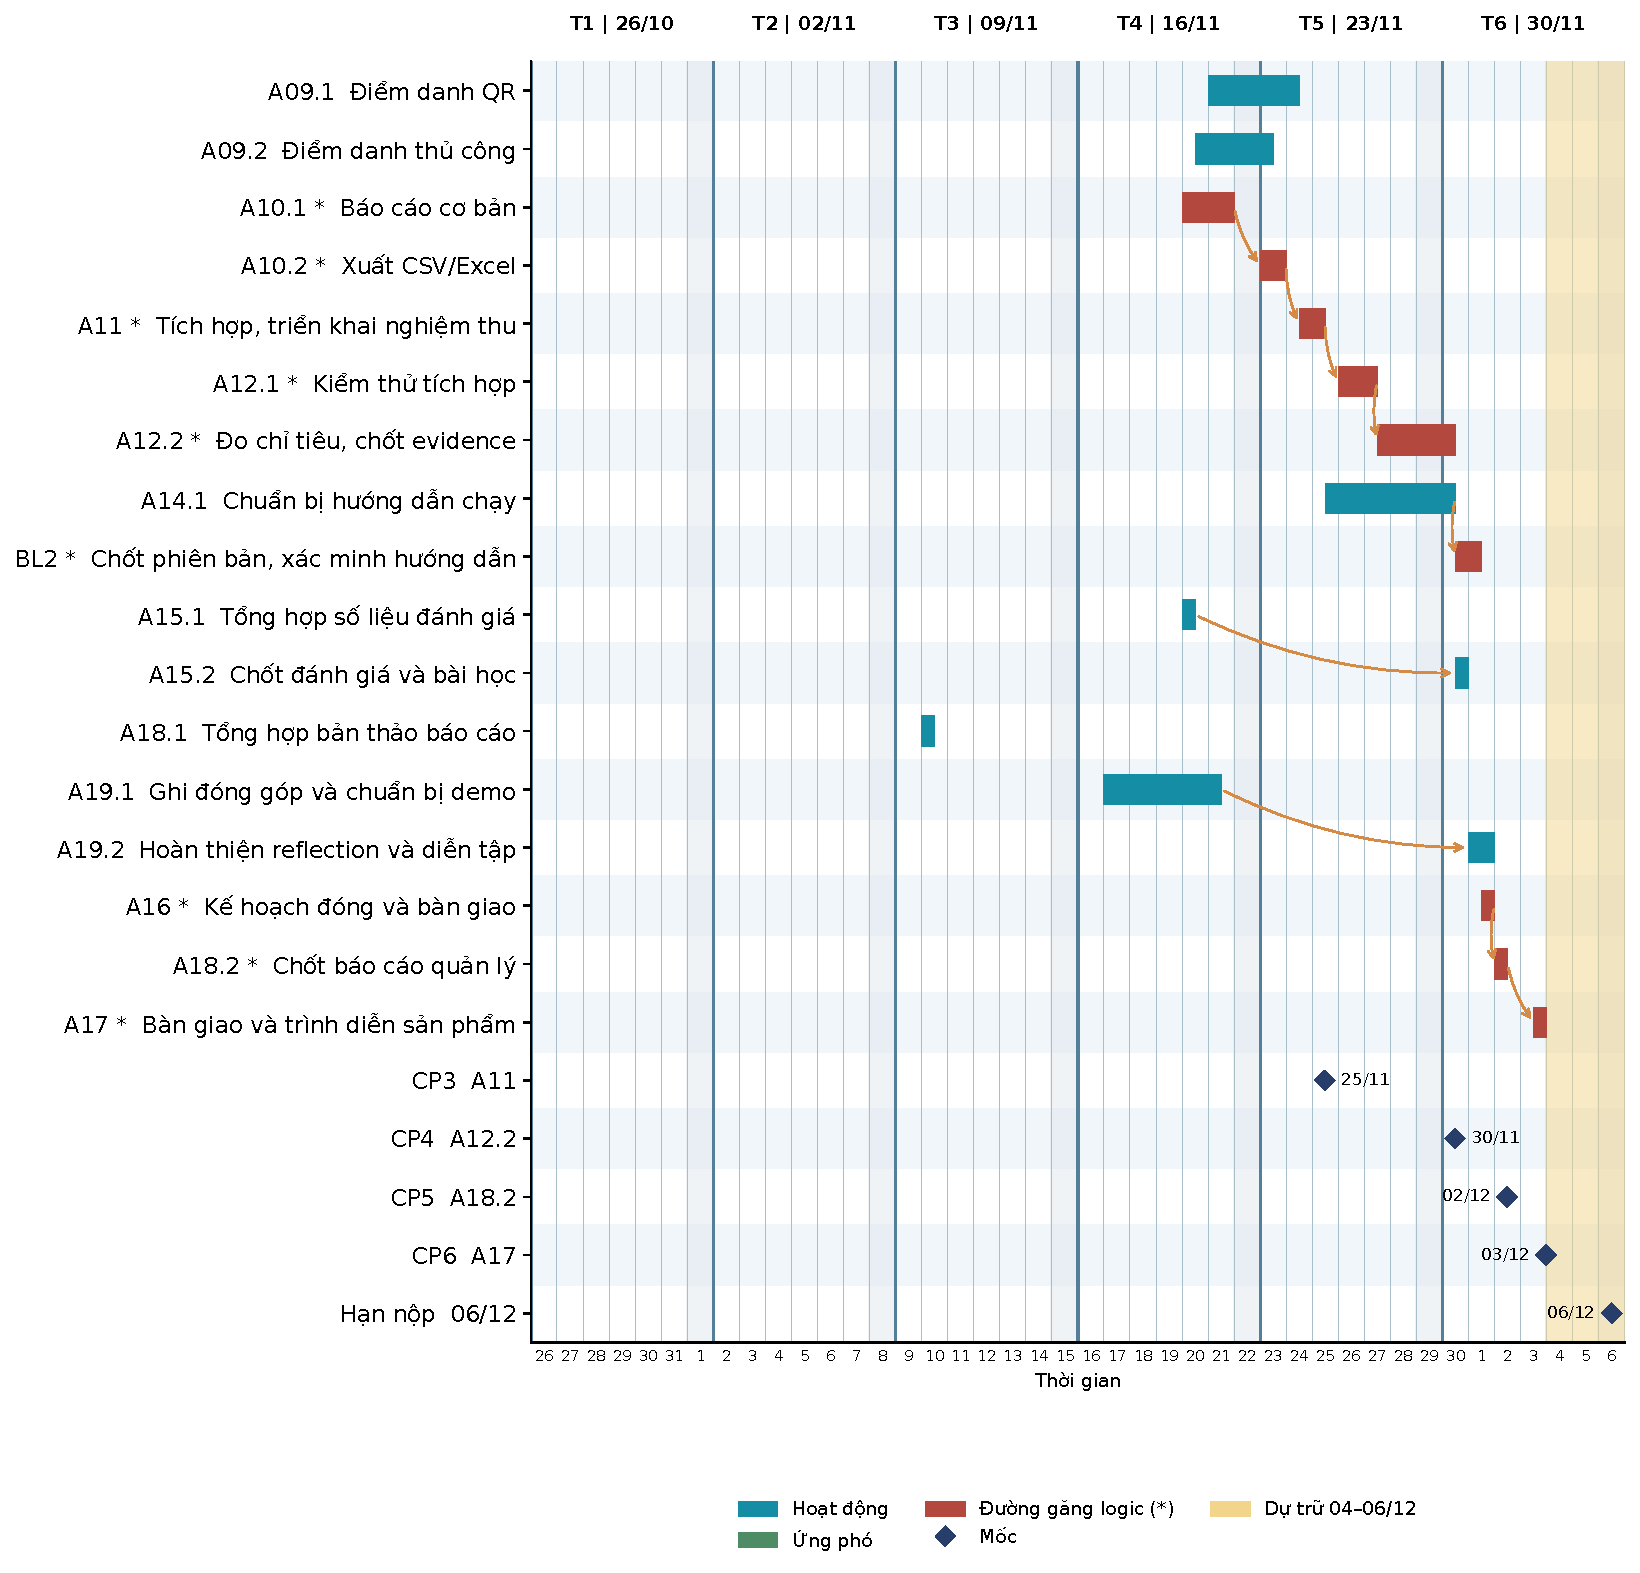
\includegraphics[width=\linewidth,height=.85\textheight,keepaspectratio]{Images/gantt_2.pdf}
\caption{Biểu đồ Gantt tiến độ Increment 3, hoàn thiện hồ sơ và bàn giao}
\label{fig:gantt2}
\end{figure}
\begin{figure}[H]
\centering
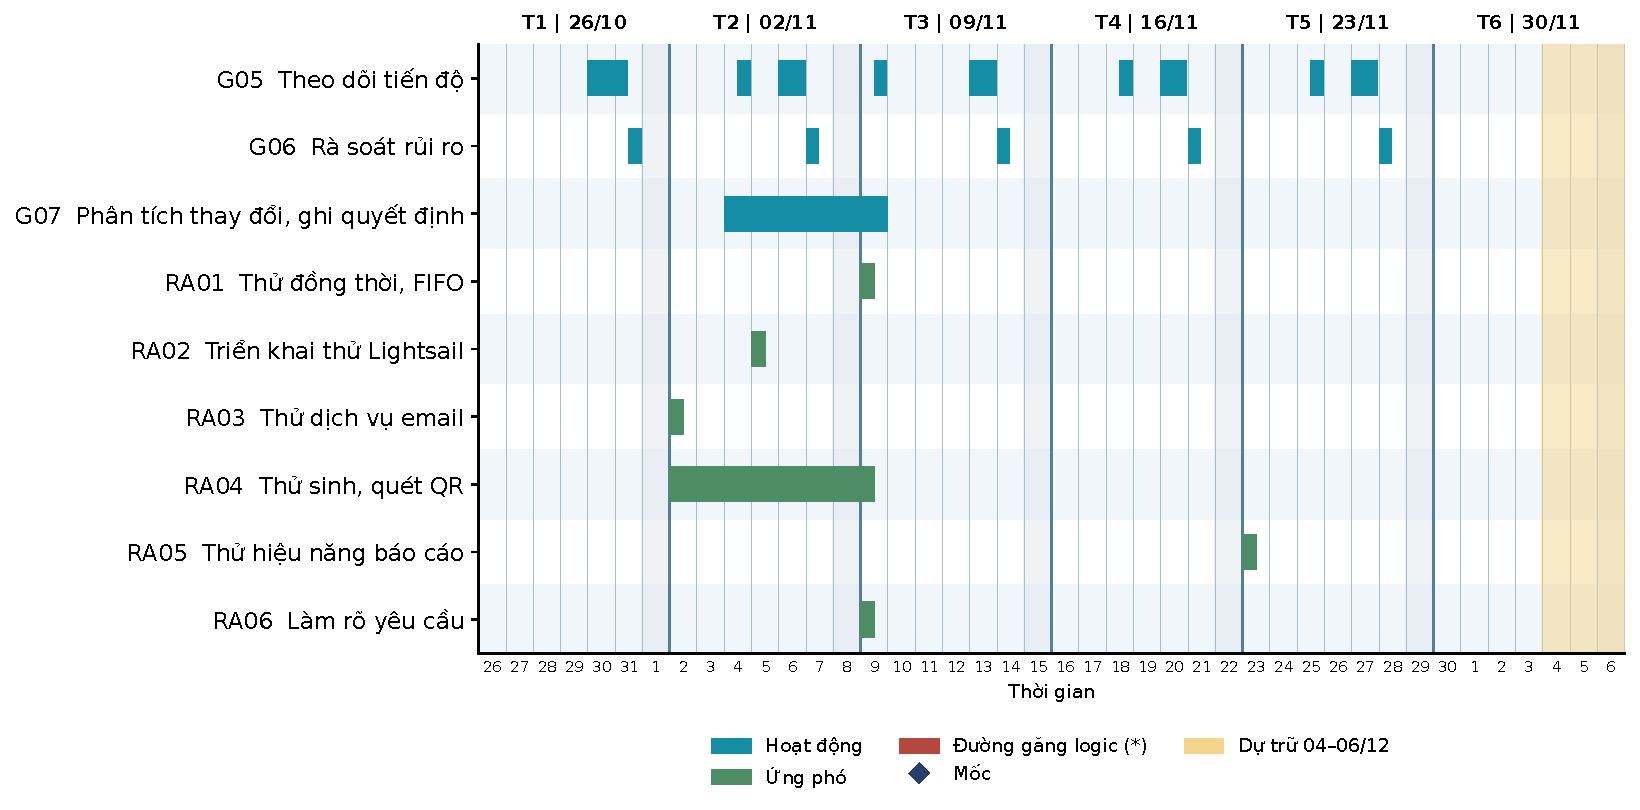
\includegraphics[width=\linewidth]{Images/gantt_ra.pdf}
\caption{Biểu đồ Gantt tiến độ các hoạt động quản lý và tác vụ rủi ro (RA)}
\label{fig:ganttra}
\end{figure}
\subsubsection{Phân tích Critical Path Method (CPM)}
Phương pháp CPM được áp dụng trên sơ đồ mạng công việc sau Activity Splitting. Thời lượng danh định $d_a$ (tính theo phiên) được xác định theo công thức:
\[
d_a=\left\lceil\frac{\max_i e_{a,i}}{2}\right\rceil,
\quad ES_a=\max_{p\in Pred(a)}EF_p,\quad EF_a=ES_a+d_a.
\]
Thuật toán duyệt lùi xác định các tham số $LF, LS$ và Total Float $TF_a = LS_a - ES_a$. Đối với gói BL2, trình tự nội bộ được bảo toàn với $d_{BL2}=2$ phiên.
Kết quả phân tích sơ đồ mạng công việc (Precedence Diagram Method - PDM) cho thấy độ dài Đường găng (Critical Path) là \textbf{47 phiên làm việc}. Chuỗi tác vụ thuộc Critical Path ($TF=0$) gồm:
\begin{quote}\small
G02 $\to$ G03 $\to$ G04 $\to$ A03 $\to$ (A05.1 hoặc A05.2) $\to$ A06 $\to$ A07.1 $\to$ A07.2 $\to$ A07.3 $\to$ A08 $\to$ A10.1 $\to$ A10.2 $\to$ A11 $\to$ A12.1 $\to$ A12.2 $\to$ BL2 $\to$ A16 $\to$ A18.2 $\to$ A17.
\end{quote}
\begin{table}[H]
\centering
\caption{Kết quả tính toán tham số CPM (Đơn vị: Phiên làm việc)}\label{tab:cpm}
\begingroup\footnotesize
\setlength{\tabcolsep}{2pt}\renewcommand{\arraystretch}{1.18}
\begin{minipage}[t]{.46\linewidth}
\vspace{0pt}\centering
\begin{tabular*}{\linewidth}{@{\extracolsep{\fill}}lrrrrrr@{}}
\toprule
\textbf{Mã} & $d$ & $ES$ & $EF$ & $LS$ & $LF$ & $TF$ \\
\midrule
A01 & 4 & 0 & 4 & 2 & 6 & 2 \\
A02.1 & 2 & 0 & 2 & 10 & 12 & 10 \\
A02.2 & 2 & 4 & 6 & 24 & 26 & 20 \\
A02.3 & 2 & 4 & 6 & 24 & 26 & 20 \\
A03 * & 2 & 6 & 8 & 6 & 8 & 0 \\
A04.1 & 1 & 4 & 5 & 12 & 13 & 8 \\
A05.1 * & 5 & 8 & 13 & 8 & 13 & 0 \\
A05.2 * & 5 & 8 & 13 & 8 & 13 & 0 \\
A06 * & 3 & 13 & 16 & 13 & 16 & 0 \\
A07.1 * & 5 & 16 & 21 & 16 & 21 & 0 \\
A07.2 * & 4 & 21 & 25 & 21 & 25 & 0 \\
A07.3 * & 2 & 25 & 27 & 25 & 27 & 0 \\
A08 * & 3 & 27 & 30 & 27 & 30 & 0 \\
A09.1 & 3 & 30 & 33 & 32 & 35 & 2 \\
A09.2 & 2 & 30 & 32 & 33 & 35 & 3 \\
A10.1 * & 3 & 30 & 33 & 30 & 33 & 0 \\
A10.2 * & 2 & 33 & 35 & 33 & 35 & 0 \\
A11 * & 2 & 35 & 37 & 35 & 37 & 0 \\
A12.1 * & 3 & 37 & 40 & 37 & 40 & 0 \\
A12.2 * & 2 & 40 & 42 & 40 & 42 & 0 \\
A14.1 & 1 & 37 & 38 & 41 & 42 & 4 \\
\bottomrule
\end{tabular*}
\end{minipage}\hfill
\begin{minipage}[t]{.46\linewidth}
\vspace{0pt}\centering
\begin{tabular*}{\linewidth}{@{\extracolsep{\fill}}lrrrrrr@{}}
\toprule
\textbf{Mã} & $d$ & $ES$ & $EF$ & $LS$ & $LF$ & $TF$ \\
\midrule
A15.1 & 1 & 30 & 31 & 42 & 43 & 12 \\
A15.2 & 1 & 42 & 43 & 43 & 44 & 1 \\
A16 * & 1 & 44 & 45 & 44 & 45 & 0 \\
A17 * & 1 & 46 & 47 & 46 & 47 & 0 \\
A18.1 & 1 & 8 & 9 & 44 & 45 & 36 \\
A18.2 * & 1 & 45 & 46 & 45 & 46 & 0 \\
A19.1 & 1 & 16 & 17 & 43 & 44 & 27 \\
A19.2 & 1 & 42 & 43 & 44 & 45 & 2 \\
BL1 & 1 & 6 & 7 & 26 & 27 & 20 \\
BL2 * & 2 & 42 & 44 & 42 & 44 & 0 \\
G02 * & 2 & 0 & 2 & 0 & 2 & 0 \\
G03 * & 3 & 2 & 5 & 2 & 5 & 0 \\
G04 * & 1 & 5 & 6 & 5 & 6 & 0 \\
G07 & 2 & 6 & 8 & 41 & 43 & 35 \\
RA01 & 1 & 8 & 9 & 20 & 21 & 12 \\
RA02 & 1 & 13 & 14 & 34 & 35 & 21 \\
RA03 & 1 & 8 & 9 & 24 & 25 & 16 \\
RA04 & 1 & 4 & 5 & 31 & 32 & 27 \\
RA05 & 1 & 33 & 34 & 39 & 40 & 6 \\
RA06 & 1 & 13 & 14 & 15 & 16 & 2 \\
\bottomrule
\end{tabular*}
\end{minipage}
\endgroup
\end{table}
\subsubsection{Đường cơ sở chi phí (Cost Baseline)}
Chi phí nhân sự tính theo đơn giá 78.000 VNĐ/giờ công; chi phí hạ tầng AWS Lightsail cố định 728.000 VNĐ cho hai kỳ thanh toán. Cost Baseline tổng thể ($B$) đã bao gồm 11,1 giờ công RA được xác định là:
\[
B = (331{,}6 \times 78.000) + 728.000 = 25.864.800 + 728.000 = \boxed{26.592.800\text{ VNĐ}}.
\]
\begingroup\small
\setlength{\tabcolsep}{4pt}\renewcommand{\arraystretch}{1.15}
\begin{longtable}{@{}p{.45\linewidth}rr@{}}
\caption{Tổng hợp chi phí theo nhân sự và khoản mục}\label{tab:costtotal}\\
\toprule
\textbf{Khoản mục} & \textbf{Tổng giờ (h)} & \textbf{Chi phí (VNĐ)} \\
\midrule\endfirsthead
\toprule
\textbf{Khoản mục} & \textbf{Tổng giờ (h)} & \textbf{Chi phí (VNĐ)} \\
\midrule\endhead
\midrule\multicolumn{3}{r}{\textit{Còn tiếp}}\\\endfoot
\bottomrule\endlastfoot
PM & 66,4 & 5.179.200 \\
BA & 62,3 & 4.859.400 \\
BE & 68,9 & 5.374.200 \\
FE & 65,0 & 5.070.000 \\
QA & 69,0 & 5.382.000 \\
\textbf{Chi phí công sức nhân sự} & \textbf{331,6} & \textbf{25.864.800} \\
Chi phí hạ tầng AWS Lightsail & --- & 728.000 \\
\textbf{Tổng Cost Baseline} & --- & \textbf{26.592.800} \\
\end{longtable}\endgroup
\begin{table}[H]
\centering
\caption{Phân bổ chi phí công sức theo từng hoạt động}\label{tab:activitycost}
\begingroup\small
\setlength{\tabcolsep}{2pt}\renewcommand{\arraystretch}{1.18}
\begin{minipage}[t]{.46\linewidth}
\vspace{0pt}\centering
\begin{tabular*}{\linewidth}{@{\extracolsep{\fill}}lrr@{}}
\toprule
\textbf{Mã} & \shortstack{\textbf{Công sức}\\\textbf{(h)}} & \shortstack{\textbf{Chi phí}\\\textbf{(VNĐ)}} \\
\midrule
A01 & 16,0 & 1.248.000 \\
A02.1 & 5,0 & 390.000 \\
A02.2 & 3,5 & 273.000 \\
A02.3 & 3,5 & 273.000 \\
A03 & 8,0 & 624.000 \\
A04.1 & 3,5 & 273.000 \\
A05.1 & 18,0 & 1.404.000 \\
A05.2 & 18,0 & 1.404.000 \\
A06 & 10,0 & 780.000 \\
A07.1 & 22,0 & 1.716.000 \\
A07.2 & 14,0 & 1.092.000 \\
A07.3 & 6,0 & 468.000 \\
A08 & 13,0 & 1.014.000 \\
A09.1 & 12,0 & 936.000 \\
A09.2 & 10,0 & 780.000 \\
A10.1 & 13,0 & 1.014.000 \\
A10.2 & 5,0 & 390.000 \\
A11 & 7,0 & 546.000 \\
A12.1 & 14,0 & 1.092.000 \\
A12.2 & 8,0 & 624.000 \\
A14.1 & 3,0 & 234.000 \\
A15.1 & 2,0 & 156.000 \\
\bottomrule
\end{tabular*}
\end{minipage}\hfill
\begin{minipage}[t]{.46\linewidth}
\vspace{0pt}\centering
\begin{tabular*}{\linewidth}{@{\extracolsep{\fill}}lrr@{}}
\toprule
\textbf{Mã} & \shortstack{\textbf{Công sức}\\\textbf{(h)}} & \shortstack{\textbf{Chi phí}\\\textbf{(VNĐ)}} \\
\midrule
A15.2 & 6,0 & 468.000 \\
A16 & 5,0 & 390.000 \\
A17 & 5,0 & 390.000 \\
A18.1 & 2,5 & 195.000 \\
A18.2 & 4,5 & 351.000 \\
A19.1 & 2,5 & 195.000 \\
A19.2 & 2,5 & 195.000 \\
BL1 & 3,5 & 273.000 \\
BL2 & 4,0 & 312.000 \\
G02 & 10,0 & 780.000 \\
G03 & 11,0 & 858.000 \\
G04 & 4,0 & 312.000 \\
G05 & 30,0 & 2.340.000 \\
G06 & 7,5 & 585.000 \\
G07 & 8,0 & 624.000 \\
RA01 & 2,5 & 195.000 \\
RA02 & 2,5 & 195.000 \\
RA03 & 1,0 & 78.000 \\
RA04 & 2,0 & 156.000 \\
RA05 & 1,9 & 148.200 \\
RA06 & 1,2 & 93.600 \\
\bottomrule
\end{tabular*}
\end{minipage}
\endgroup
\end{table}

Tổng công sức của các hoạt động là 331,6 giờ công, tương ứng chi phí nhân sự 25.864.800 VNĐ.

\begingroup\small
\setlength{\tabcolsep}{3pt}\renewcommand{\arraystretch}{1.15}
\begin{longtable}{@{}lrrrrr@{}}
\caption{Bảng phân bổ chi phí kế hoạch theo tuần (Dòng tiền dự án)}\label{tab:weeklycost}\\
\toprule
\textbf{Tuần} & \shortstack{\textbf{Công}\\\textbf{sức (h)}} & \shortstack{\textbf{Chi phí}\\\textbf{nhân sự}} & \shortstack{\textbf{Chi phí}\\\textbf{hạ tầng}} & \shortstack{\textbf{Chi}\\\textbf{phí tuần}} & \shortstack{\textbf{Chi phí}\\\textbf{lũy kế}} \\
\midrule\endfirsthead
\toprule
\textbf{Tuần} & \shortstack{\textbf{Công}\\\textbf{sức (h)}} & \shortstack{\textbf{Chi phí}\\\textbf{nhân sự}} & \shortstack{\textbf{Chi phí}\\\textbf{hạ tầng}} & \shortstack{\textbf{Chi}\\\textbf{phí tuần}} & \shortstack{\textbf{Chi phí}\\\textbf{lũy kế}} \\
\midrule\endhead
\midrule\multicolumn{6}{r}{\textit{Còn tiếp}}\\\endfoot
\bottomrule\endlastfoot
T1 & 63,5 & 4.953.000 & 364.000 & 5.317.000 & 5.317.000 \\
T2 & 64,0 & 4.992.000 & 0 & 4.992.000 & 10.309.000 \\
T3 & 61,1 & 4.765.800 & 0 & 4.765.800 & 15.074.800 \\
T4 & 60,2 & 4.695.600 & 0 & 4.695.600 & 19.770.400 \\
T5 & 53,4 & 4.165.200 & 364.000 & 4.529.200 & 24.299.600 \\
T6 & 29,4 & 2.293.200 & 0 & 2.293.200 & 26.592.800 \\
\textbf{Tổng} & \textbf{331,6} & \textbf{25.864.800} & \textbf{728.000} & \textbf{26.592.800} & --- \\
\end{longtable}\endgroup
\begin{figure}[H]
\centering
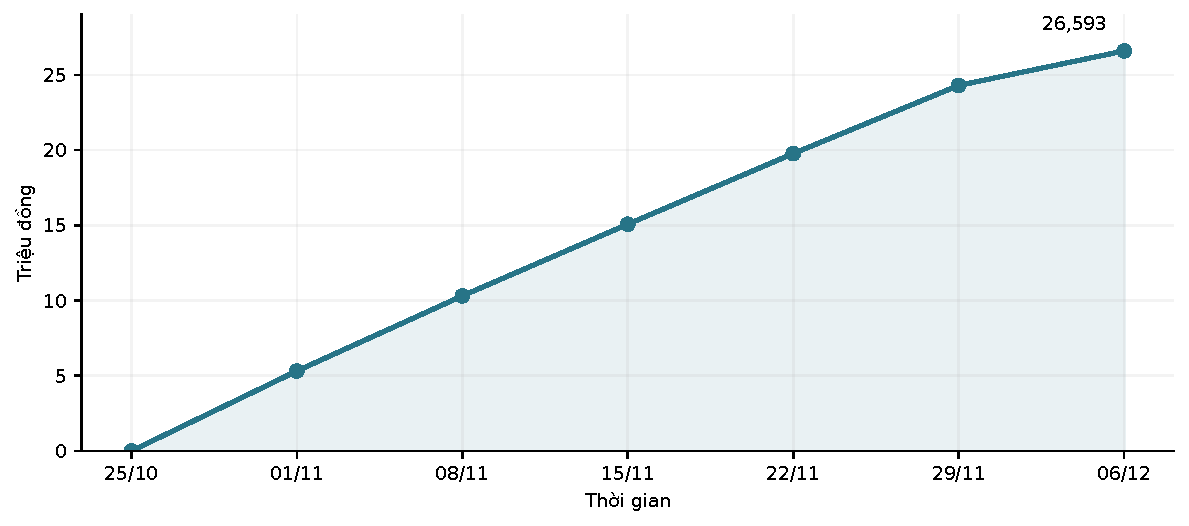
\includegraphics[width=\linewidth]{Images/chi_phi.pdf}
\caption{Đường cong chi phí kế hoạch lũy kế (S-Curve Cost Baseline)}
\label{fig:cost}
\end{figure}
Hình \ref{fig:cost} minh họa S-Curve của Cost Baseline từ mốc 0 VNĐ (ngày 25/10/2026) đạt mốc 26.592.800 VNĐ tại Tuần 6.